

\subsection{Gaussian Beam}

\begin{figure}[h!]
    \centering

    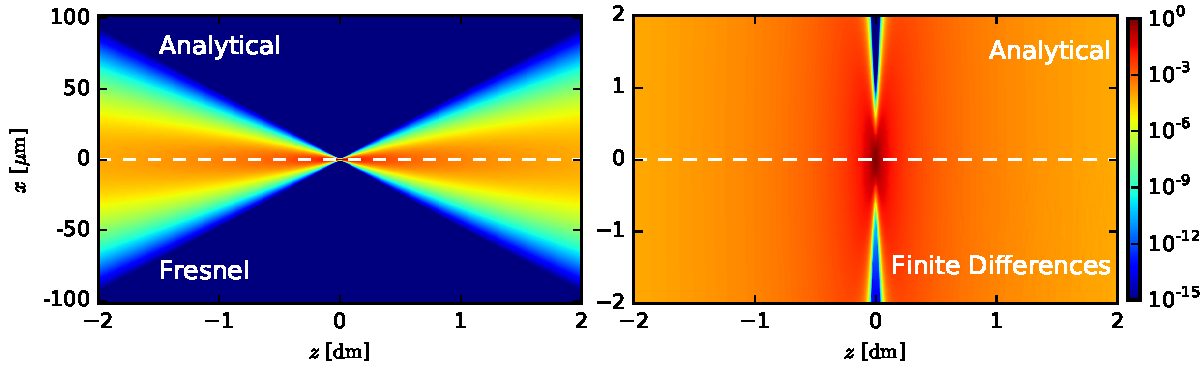
\includegraphics[width=1\textwidth]{analytical/analytical_gauss_fdfr}
    
    \caption{Normalized intensity cross-section of a Gaussian beam with a waist size of $250\text{nm}$ propagated with the Fresnel propagator (Left) and the finite difference propagator (Right) compared to the analytical solution. Note how the simulation box size of the finite difference propagator can be chosen much smaller as the beam can \emph{shine} in and out from the analytical solution through the boundary conditions. In both cases the maximal deviation from the analytical solution is less than $1\%$ of the field strength in the focal point.}
    
    %Ceneter: Normalized intensity cross-section of a Gaussian beam with a waist size of $1 \mu\text{m}$ which is rotated by 4$\text{m} \text{deg}$ propagated with the Finite Difference propagator using the analytical beam values at the boundaries. Right: The largest absolute difference of the Finite Difference propagated beam to the analytical Gaussian beam as a function of the rotation angle $\varphi$. The simulation box was chosen in a way that the beam propagated for 10cm and the focus was in the center.
    
    \label{fig:gauss_analytical_comparison}
\end{figure}


\subsubsection{Analytical solution}

One of the most fundamental analytical solutions to the paraxial wave equation is the Gaussian beam, which exhibits a Gaussian intensity profile in $xy$ direction. At $z = 0$ the field of the Gaussian beam is given by

\begin{align*}
    \psi_\text{Gauss}(r,0) = \psi_0 \; \text{exp}  \mathopen{} \left(-\frac{ r^2 }{{w_0}^{2}} \right) \mathclose{},
\end{align*}

where $r = \sqrt{x^2 + y^2}$ is the distance from the $z$ axis, $\psi_0 = \psi_\text{Gauss}(0,0)$ is the field strength in the focal point and $w_0$ is the initial waist size of the beam. Using equation \eqref{eq:fresnel_convolution} we find the analytical solution for the Gaussian beam for all $z$ as a convolution with the elementary solution of the paraxial wave equation. Evaluating the integral and setting $n = 1$ we find

\begin{align*}
    \psi_\text{Gauss}(r,z) = \psi_0 \; \text{exp} \mathopen{} \left(i k z -\frac{ r^2 }{{w_r(z)}^{2}} \right) \mathclose{} \; \frac{w_0^2}{w_r(z)^2} ,
\end{align*}

where $w_r(z) = \sqrt{2iz/k + w_0^2}$ is the complex beam waist size.

\subsubsection{Solution by Fresnel propagation}

We use the Fresnel propagator to propagate the field of a Gaussian beam with parameters $w_0 = 250\text{nm}$ at $z_\text{min} = -200\mathrm{mm}$ from $z_\text{max} = 200\mathrm{mm}$. Since the implementation of the Fresnel propagator requires periodic boundary conditions, we must choose the simulation box large enough that almost all intensity is contained inside. We therefore choose $x_\text{max} = y_\text{max} = |x_\text{min}| = |y_\text{min}| = 204 \mu\text{m}$ since this gives us field amplitudes of less than $10^{-8} \psi_0$ at the box boundaries. In \figref{fig:gauss_analytical_comparison} (Left) we can see a comparison of the propagated intensities with the analytical solution. For more details see \lstinline{gaussian.ipynb} in the supplemental material.


\subsubsection{Solution by Finite Difference propagation}

Since we can specify the field values at the boundaries it is possible to \emph{shine in} the beam through the simulation box boundaries. This gives us much higher flexibility when formulating our simulations allowing to propagate smaller segments or rotated beams while keeping a reasonably sized simulation box.  In \figref{fig:gauss_analytical_comparison} (Right) we can see a comparison of the propagated intensities with the analytical solution. For more details see \lstinline{gaussian.ipynb} in the supplemental material.









